\documentclass[11pt]{article}
\usepackage{amsmath,amsthm,amssymb,fullpage,graphicx,hyperref,listings}
\usepackage{listings,color,setspace}
\author{Andy Reagan}
\title{Math 337 Homework 08}

     \def\NN{\mathbb{N} }
     \def\ZZ{\mathbb{Z} }
     \def\QQ{\mathbb{Q} }
     \def\RR{\mathbb{R} }
     \def\CC{\mathbb{C} }
     \def\f{\frac }
     \def\b{\begin }
     \def\e{\end }
     \def\Log{\text{Log} \,}
     \def\Re{\text{Re} \, }

\lstset{language=MATLAB,
basicstyle=\ttfamily\scriptsize\singlespacing,
keywordstyle=\color{black},
stringstyle=\color{black},
commentstyle=\color{black},
morecomment=[l][\color{black}]{\#},
frame=L,
xleftmargin=\parindent,
%%numbers=left,                   %% where to put the line-numbers
%%numberstyle=\scriptsize,      %% the size of the fonts that are used for the line-numbers
%%stepnumber=1,                   %% the step between two line-numbers. If it is 1 each line will be numbered
numbersep=5pt,
breaklines=true,        %% sets automatic line breaking
breakatwhitespace=false,    %% sets if automatic breaks should only happen at whitespace
escapeinside={\%*}{*)} 
}


     \newcommand{\pdiff}[2]{\frac{\partial #1}{\partial #2}}
     \newcommand{\partialdiff}[2]{\frac{\partial #1}{\partial #2}}
     \newcommand{\pdiffsq}[2]{\frac{\partial^2 #1}{{\partial #2}^2}}
     \newcommand{\pdiffcu}[2]{\frac{\partial^3 #1}{{\partial #2}^3}}
     \newcommand{\pdiffhi}[3]{\frac{\partial^#3 #1}{{\partial #2}^#3}}
     \newcommand{\diff}[2]{\frac{{\rm d}#1}{{\rm d}#2}}
     \newcommand{\diffsq}[2]{\frac{{\rm d}^{2}#1}{{\rm d} {#2}^2}}
     \newcommand{\diffhi}[3]{\frac{{\rm d}^#3 #1}{{\rm d} {#2}^#3}}
     \newcommand{\tdiff}[2]{\mbox{d} #1/\mbox{d} #2}
     \newcommand{\tdiffsq}[2]{\mbox{d}^{2} #1/\mbox{d} {#2}^2}
     \newcommand{\tpdiff}[2]{\partial #1/\partial #2}
     \newcommand{\tpdiffsq}[2]{\partial^2 #1/\partial {#2}^2}
     \newcommand{\bvec}[1]{\vec{ {\bf #1 } }}
     \newcommand{\oh}[1]{O(h^{{#1}})}

\begin{document}
\maketitle

\begin{enumerate}

\item Use the Gerschgorin Circles Theorem and the fact that the eigenvalues of real symmetric matrices are real to obtain the best estimate for the location of the eigenvalues of the following tri-diagonal matrix:
\[ A = \left ( \begin{array}{ccccccc} a & -1 & 0 & . & . & . & 0\\
-1 & a & -1 & 0 & . & . & 0\\
0 & -1 & a & -1 & 0 & . & 0\\
 &  &  & . & . & . & \\
0 & . & . & 0 & -1 & a & -1\\
0 & . & . & . & 0 & -1 & a\end{array} \right ) , \]
where $a$ is a real number.
In particular, what is the minimum distance between an eigenvalue of this matrix and zero?

\bigskip
\textbf{Solution:} By the Gerschgorin Circles Theorem, all of the eigenvalues are found in circles centered at $a$.
The radius of these circles is $1$, corresponding to the first and last rows, and $2$ otherwise.
Since the eigenvalues are real, we know that they fall in the interval $[a-2,a+2]$ on the real line.

In particular, the distance between the eigenvalues of this matrix and 0 is at least $a-2$ if $a>2$ and $a+2$ is $a<2$. If $|a|\leq 2$, the minimum distance is 0 (i.e., the eigenvalues can well be 0).

%% My code and a solution plot follow.

%% \lstinputlisting[language=Matlab]{andy_hw08_prb01.m}

%% \begin{figure}[h!]
%%   \centering
%%     \includegraphics[width=0.5\textwidth]{andy_hw08_prb01_01.pdf}
%%   \caption{Solution of the BVP with the shooting method.}
%% \end{figure}

\item Consider a linear BVP
\[ y'' + 2(2-x)y' = 2(2-x), y(0) = -1, y(6) = 5.\]
Discretize it using scheme (8.4) with $h = 1$.
\begin{enumerate}

\item[(i)] Verify that you obtain a linear system
\[ \left ( \begin{array}{ccccc} -2 & 2 & 0 & 0 & 0\\
1 & -2 & 1 & 0 & 0\\
0 & 2 & -2 & 0 & 0\\
0 & 0 & 3 & -2 & -1\\
0 & 0 & 0 & 4 & -2\end{array} \right ) \left (\begin{array}{c} Y_1 \\
Y_2\\
Y_3\\
Y_4\\
Y_5\end{array} \right ) = \left (\begin{array}{r} 2 \\
0\\
-2\\
-4\\
4\end{array} \right ).\]

\item[(ii)] Solve is using MATLAB. What do you obtain?
\item[(iii)] The result you have obtain in part (ii) occurs because one of the conditions of Theorem 8.3 is violated.
What is the condition?
\end{enumerate}

\bigskip
\textbf{Solution:} 
\begin{enumerate}
\item[(i)] For this problem, equation (8.4) becomes
\begin{align} &Y_0 = -1;\\
&(1+h(2-x_n))Y_{n+1} -2 Y_n + (1-h(2-x_n)) Y_{n-1} = 2 h^2 (2-x_n),~~~1\leq n \leq 5 \label{eq:11}\\
&Y_6 = 5.\end{align}
Setting $h = 1$ in \eqref{eq:11}, this become
\begin{equation} (3-x_n)Y_{n+1} -2 Y_n + (-1+x_n) Y_{n-1} = 4-2x_n; \label{eq:11}\end{equation}
We have the following 5 discrete equations for $Y_{1\ldots 5}$, where $Y_0$ and $Y_6$ are the supplied BC.
\begin{align*} (3-x_1)Y_{2} -2 Y_1 + (-1+x_1) Y_{0} = 4-2x_1; \\
(3-x_2)Y_{3} -2 Y_2 + (-1+x_2) Y_{1} = 4-2x_2; \\
(3-x_3)Y_{4} -2 Y_3 + (-1+x_3) Y_{2} = 4-2x_3; \\
(3-x_4)Y_{5} -2 Y_4 + (-1+x_4) Y_{3} = 4-2x_4; \\
(3-x_5)Y_{6} -2 Y_5 + (-1+x_5) Y_{4} = 4-2x_5. \end{align*}
Plugging in $x_i = i$ and $Y_0 = -1, Y_6 = 5$, and moving constants to the RHS, we are left
\begin{align*} 2Y_{2} -2 Y_1 = 2; \\
Y_{3} -2 Y_2 + Y_{1} = 0; \\
-2 Y_3 + 2Y_{2} = -2; \\
-Y_{5} -2 Y_4 + 3Y_{3} = -4; \\
-2 Y_5 + 4Y_{4} = 4. \end{align*}
Intuitively obvious to the casual observer, this agrees with the desired linear system.

\item[(ii)] MATLAB obtain a vector of all NaN's, the matrix being singular to working precision.

\lstinputlisting[language=Matlab]{andy_hw08_prb02.m}

\item[(iii)] The requirement of Theorem 8.3 that $h\mathcal{P} \leq 2$ is violated.
Here $P(x)$ achieves a magnitude of 8, at $x = 6$, and we had chose $h = 1$.
Therefore, our $h\mathcal{P} = 8$.
\end{enumerate}


\item 
\begin{enumerate}
\item Give an operation count for finding $L$ and $U$ for a tridiagonal matrix, as per Eq. (8.21).
\item Give operation counts for solving the systems in (8.17), as per (8.22) and (8.23). 
\item Given the total operations count for the Thomas algorithm.
\end{enumerate}

\bigskip
\textbf{Solution:} 
\begin{enumerate}
\item We compute $M-1$ new $\alpha$ values, and $M-1$ new $\beta$ values.
Each new $\alpha$ requires one operation, and each $\beta$ requires 2.
Therefore, we use $3(M-1)$ operations.
\item Solving for $\vec{z}$ requires exactly $2(M-1)$ operations.
The solving for $\vec{y}$ requires exactly $1+3(M-1)$ operations.
In total, this is $1+5(M-1)$ operations.
\item The total operation count is (adding the two previous counts) $1+8(M-1)$.
\end{enumerate}

\clearpage
\pagebreak
\item Use the \verb|thomas.m| function, posted under ``Codes for examples and selected homework problems,'' to solve a tridiagonal system $A\vec{y} = \vec{r}$ where $A$ has '2' on the main diagonal and '-1' on the two subdiagonals.
Take $\vec{r} = [1,-1,1,-1,\ldots]^T$ and $M = 1000$ and 5000.
Now solve the same system using Matlab's solver.
Here, you need to investigate {\em two} cases: One, when $A$ is constructed as a regular (i.e., full) matrix and two, when it is constructed as a sparse matrix.

Compare the computational times required to solve this system for your code and for the MATLAB's solver, in those two cases.
In particular, comment on {\em how the computational times scale with $M$} in each of the three cases considered.

\bigskip
\textbf{Solution:} I compare with the following code, and plot how the computational times scale with $M$ (using more values of $M$).
I find that both the \verb|thomas.m| code and MATLAB's sparse solver scale linearly with $M$, with MATLAB's solver being faster.

For a non-sparse matrix, MATLAB's solver scales superlinearly (perhaps quadraticaly) with $M$, and becomes useless quickly.

\lstinputlisting[language=Matlab]{andy_hw08_prb04.m}

\begin{figure}[h!]
  \centering
    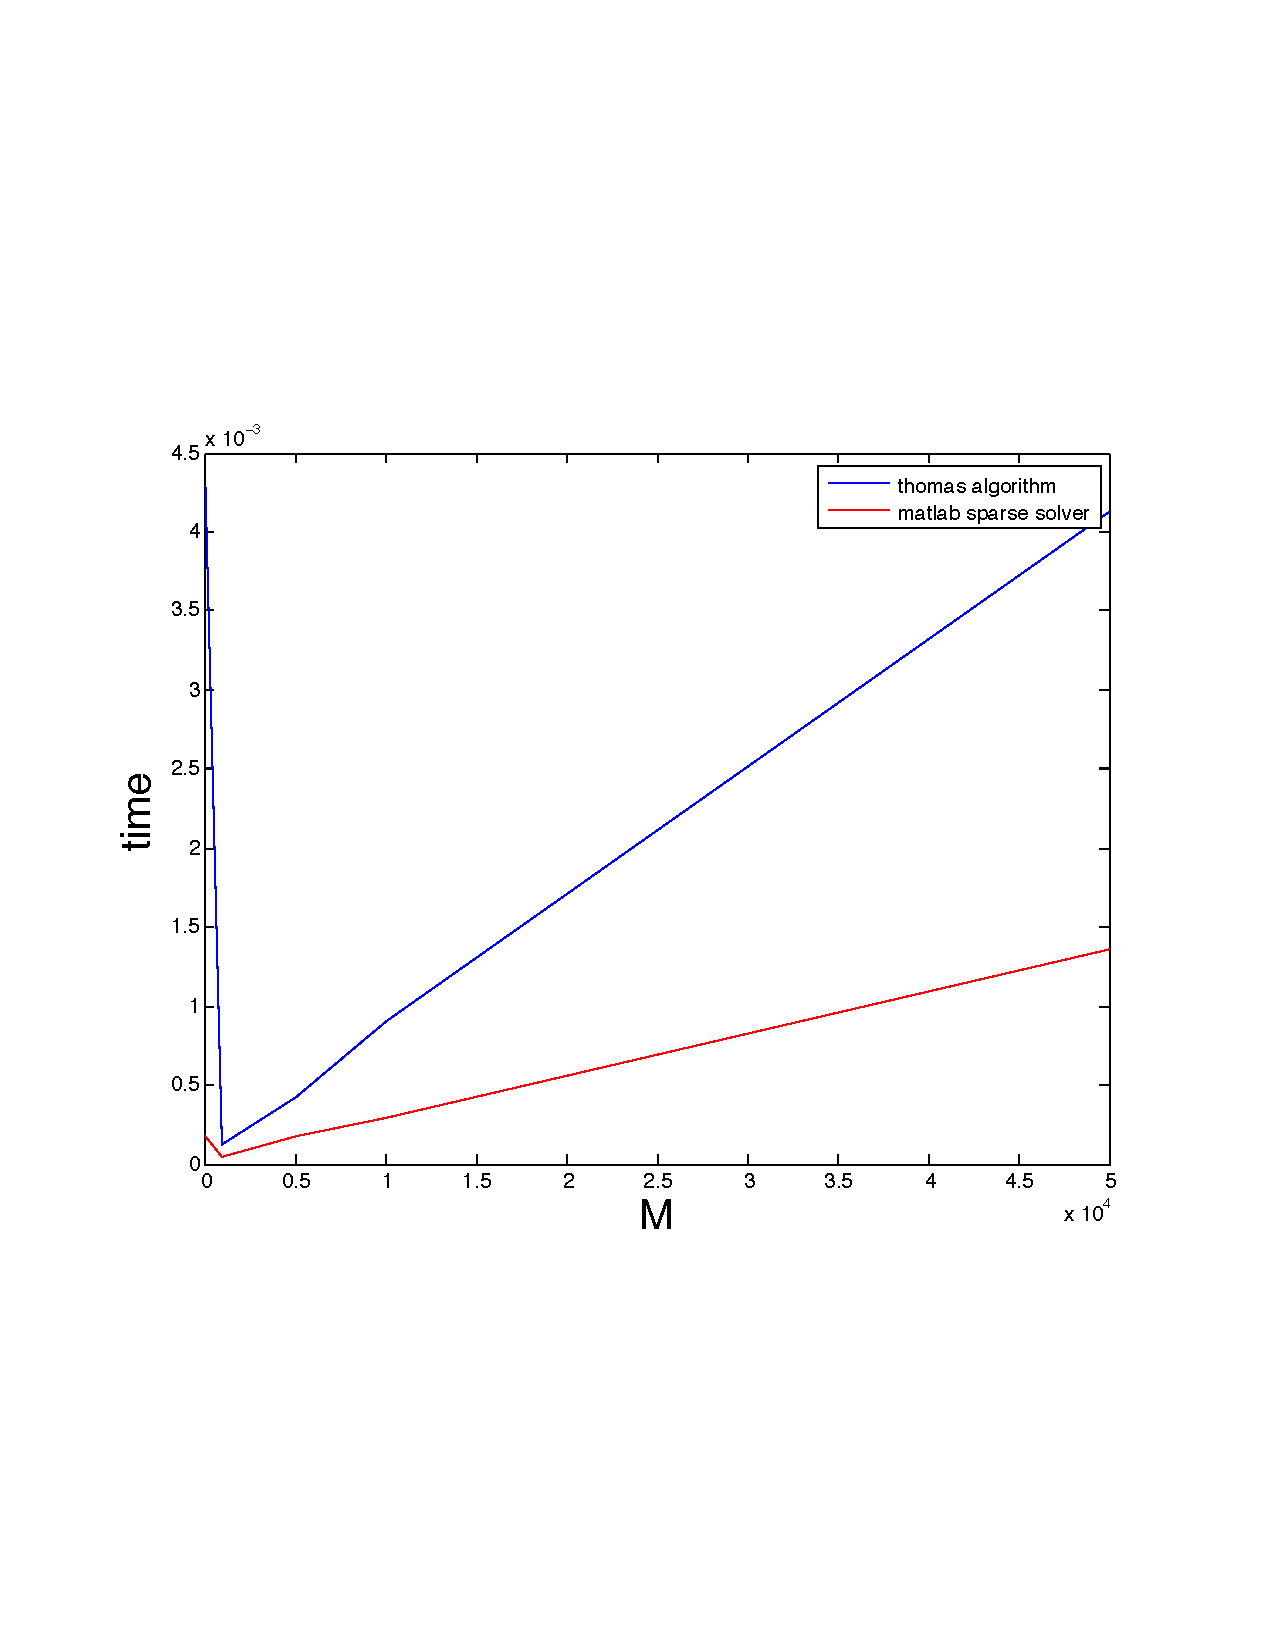
\includegraphics[width=0.5\textwidth]{andy_hw08_prb04_01.pdf}
  \caption{Scaling of computational time for thomas.m and MATLAB's built in solver, with a sparse matrix, versus $M$.}
\end{figure}

\begin{figure}[h!]
  \centering
    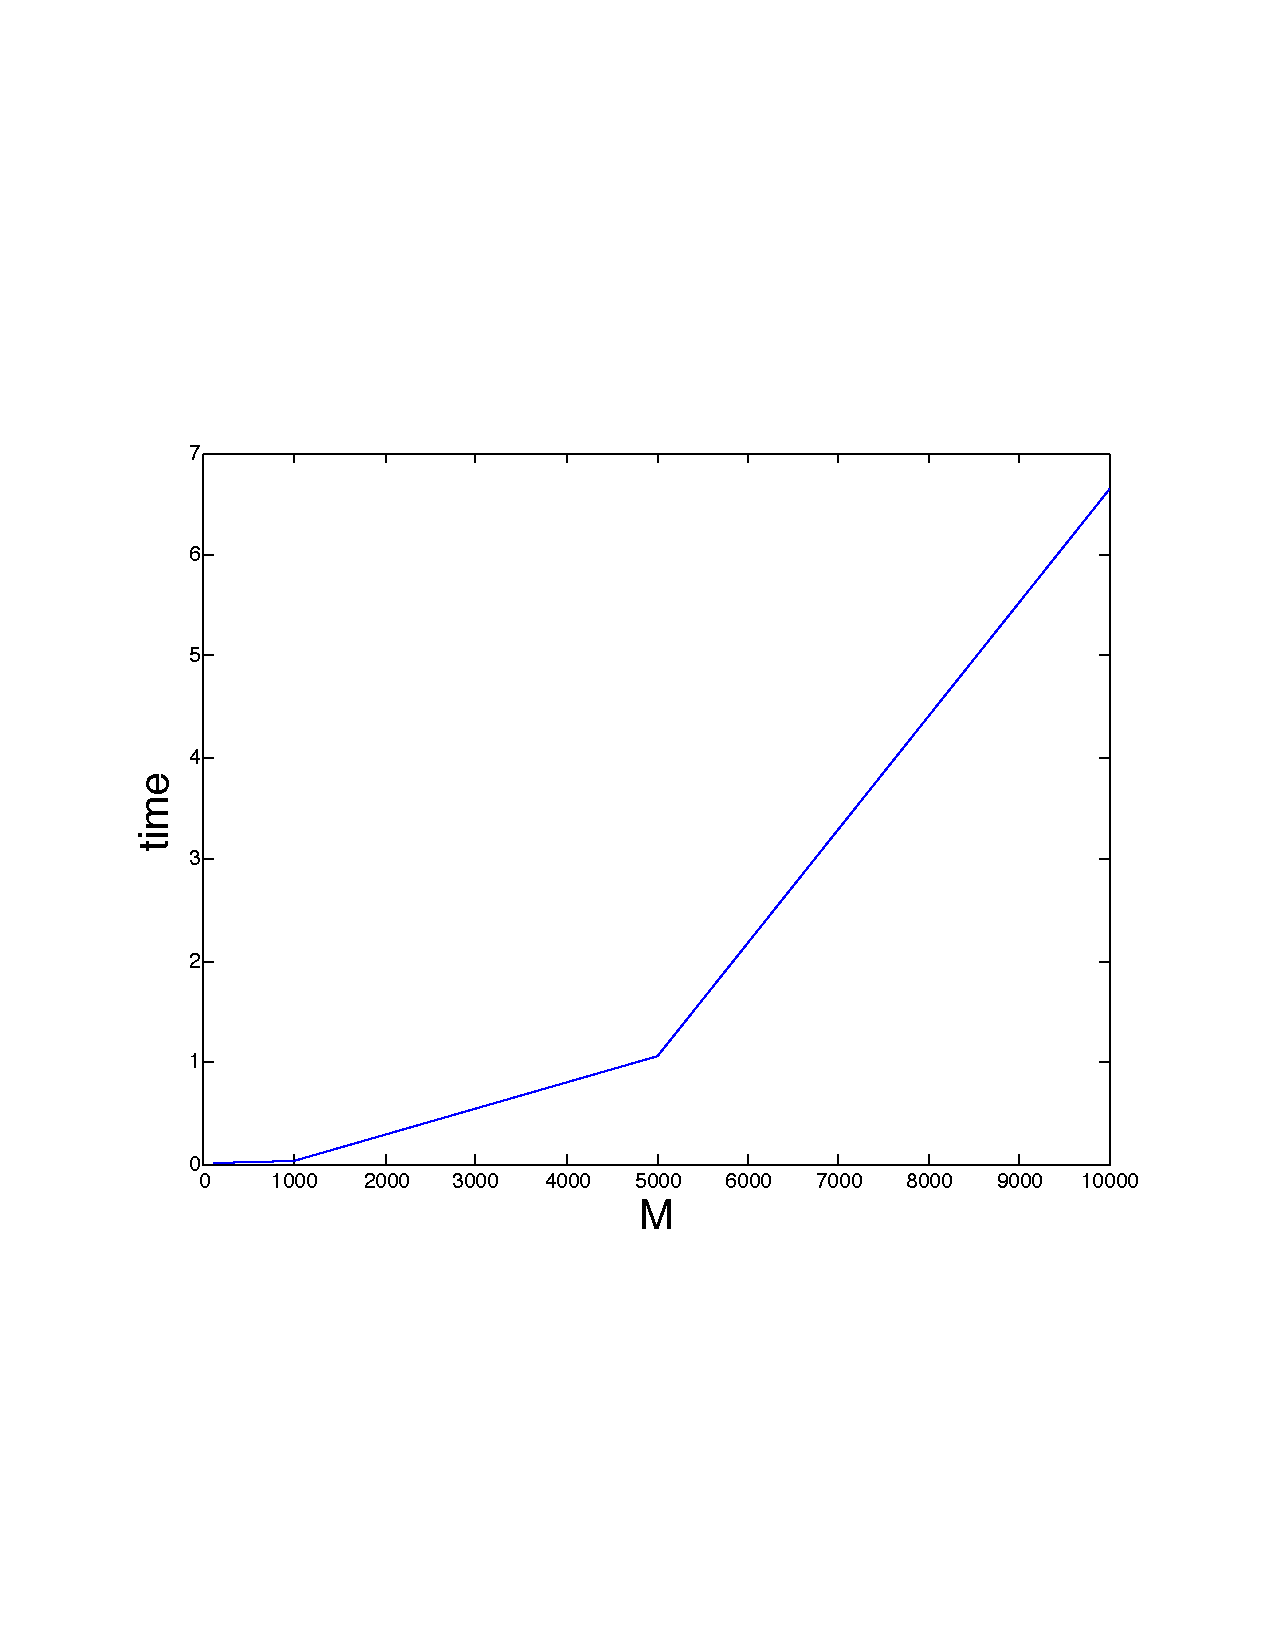
\includegraphics[width=0.5\textwidth]{andy_hw08_prb04_02.pdf}
  \caption{Scaling of computational time for MATLAB's built in solver, with a non-sparse matrix, versus $M$. It is impractical on a personal computer to extend $M$ much further than a 10,000 by 10,000 matrix, which takes 7 second to solve.}
\end{figure}

\clearpage
\pagebreak
\item Redo Problem 4 of HW07 using the discretized BVP (8.4) with $h = 0.09$ (ste size $h = 0.1$ will not ``fit'' into the interval $[0,1.62]$).
Compare the result with that found in HW07.
Which method, shooting or finite-difference discretization, is preferable for solving BVPs like this one?
\begin{enumerate}
\item[Bonus (a)] Plot the error of your numerical solution. Explain the result.
\item[Bonus (b)] Repeat the problem with $h = 0.01$ and plot the error. Explain why it is greater than that for $h = 0.09$.
\end{enumerate}

\bigskip
\textbf{Solution:} The problem is
\begin{align*} y'' = 30^2 (y - 1 + 2x), ~~~~y(0) = 1, ~~~~y(1.62) = -2.24.\end{align*}
Discretizing using (8.4) is 
\begin{align*} &Y_0 = 1;\\
&Y_{n+1} - Y_n (2-30^2h^2) + Y_{n-1} = 30^2 h^2 (2x_n -1 ) , ~~~1\leq n \leq N-1;\\
&Y_N = -2.24\end{align*}
I build this matrix in MATLAB and solve it using the built in solver.

Clearly, the finite-difference discretization is preferable to (sinlge) shooting for BVP like this one.

\lstinputlisting[language=Matlab]{andy_hw08_prb05.m}

\begin{figure}[h!]
  \centering
    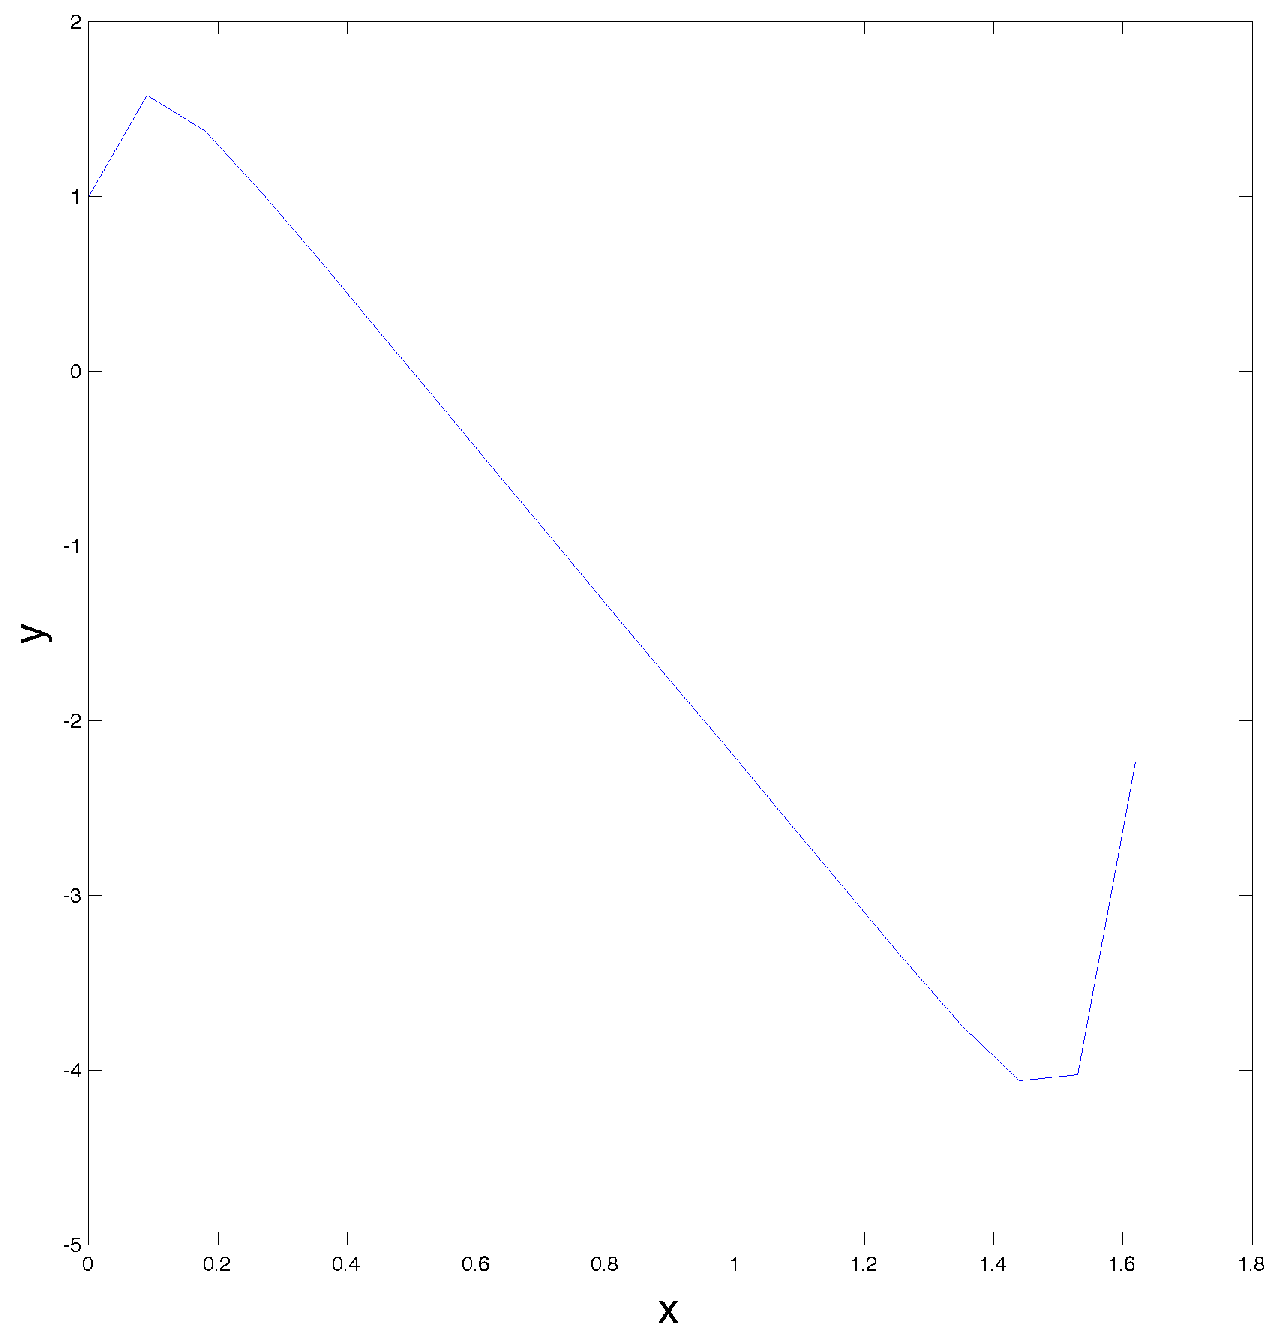
\includegraphics[width=0.5\textwidth]{andy_hw08_prb05_01.pdf}
  \caption{Solution the HW07 problem 4, using the finite difference scheme given by Eq (8.4).}
\end{figure}

\begin{figure}[h!]
  \centering
    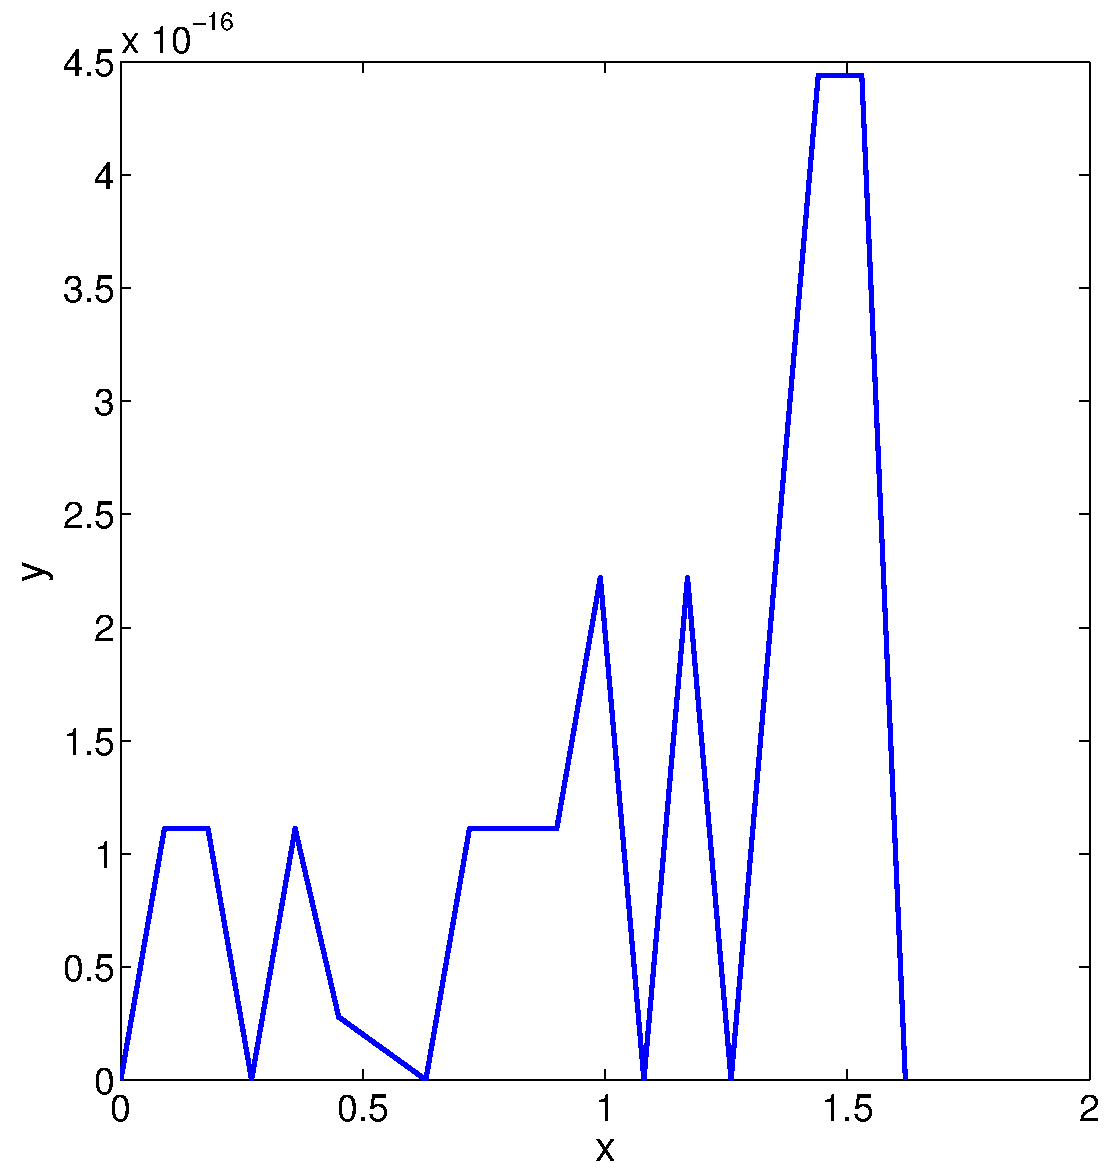
\includegraphics[width=0.5\textwidth]{andy_hw08_prb05_error.pdf}
  \caption{Error in the solution to HW07 problem 4, using the finite difference scheme given by Eq (8.4). The error is on the order of machine order, since the solver does not encounter large round-off errors from how the $30^2$ enter the matrix.}
\end{figure}

\begin{figure}[h!]
  \centering
    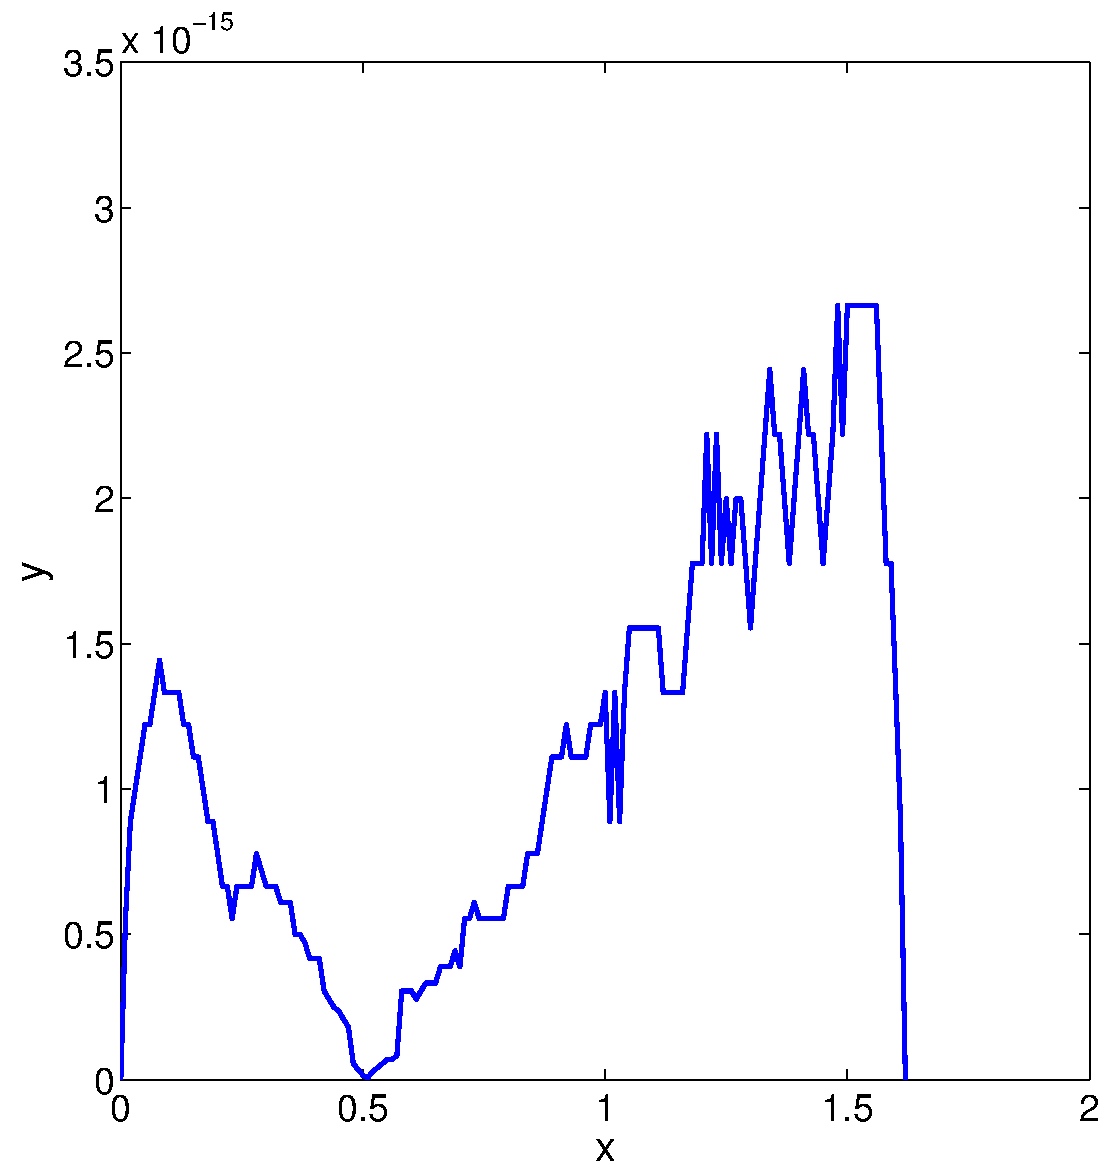
\includegraphics[width=0.5\textwidth]{andy_hw08_prb05_errorsmall.pdf}
  \caption{Error in the solution to HW07 problem 4, using the finite difference scheme given by Eq (8.4). We now use $h=0.01$, and note that error is larger than for $h=0.09$. A possible explanation for this could be that the $30^2$ represented on the computer is made much smaller when multiplied by $h^2 = 10^{-4}$, resulting in a loss of precision.}
\end{figure}

\clearpage
\pagebreak
\item Solve the BVP
\[ (1+x)^2 y'' = 2y-4 , ~~~~y(0) =  0, ~~~~y(1) + 2y'(1) = 2 \]
using the second-order accurate discretization (8.4) (for $n = 1,\ldots,N-1$) of this BVP.
Use Method 1 of Sec. 8.4 modified in such a way that it can handle the mixed type BC at the {\em right} end point of the interval.

Confirm that you numerical solution has the second order of accurarcy by comparing it at different $h$ with the exact solution $y_\text{exact} = 2x/(1+x)$.
For this, do the following:
\begin{enumerate}
\item[(i)] Run your code with $h = 0.05$ and $h = 0.025$;
\item[(ii)] Plot the error as a function of $x$;
\item[(iii)] Confirm that the maximum error scales as $O(h^2)$.
\end{enumerate}

\bigskip
\textbf{Solution:} To account for the mixed BC,
\[ A_1 y(b) + A_2 y'(b) = \beta,\]
we introduce the point $Y_{N+1}$ and approximate $y'(b)$ with a second order approximation
\[y'(b) = \f{Y_{N+1}-Y_{N-1} }{2h} + \oh{2} .\]
The mixed BC is therefore discretized as
\begin{equation} A_1 Y_{N} + A_{2} \f{Y_{N+1}-Y_{N-1} }{2h} = \beta. \label{eq:disBC}\end{equation}
The ODE discretized at $x_N$ is
\begin{equation} \left ( 1+P_N \right ) Y_{N+1} - \left ( 2 - h^2 Q_N \right ) Y_N + \left ( 1 - \f{h}{2} P_N \right ) Y_{N-1} = h^2 R_{N} \label{eq:disODE} \end{equation}
Solving for $Y_{N+1}$ in \eqref{disBC} into \eqref{disODE} we have
\begin{equation} - \left ( 2 - h^2 Q_N + 2h \f{A_1}{A_2} \left ( 1 + \f{h}{2} P_N \right ) \right ) Y_N + 2 Y_{N-1} = h^2 R_{N}- \left ( 1+ \f{h}{2}P_N\right ) \f{2h\beta}{A_2}  \label{eq:disODEnew} \end{equation}
where the first two terms on the LHS and the last term on the RHS make these matrix diagonal entries different.
I solve this in MATLAB, and plot the error versus $h$.
We find that the maximum error increases fourfold when $h$ is doubled, confirming that the method is $\oh{2}$ accurate.

\lstinputlisting[language=Matlab]{andy_hw08_prb06.m}

\begin{figure}[h!]
  \centering
    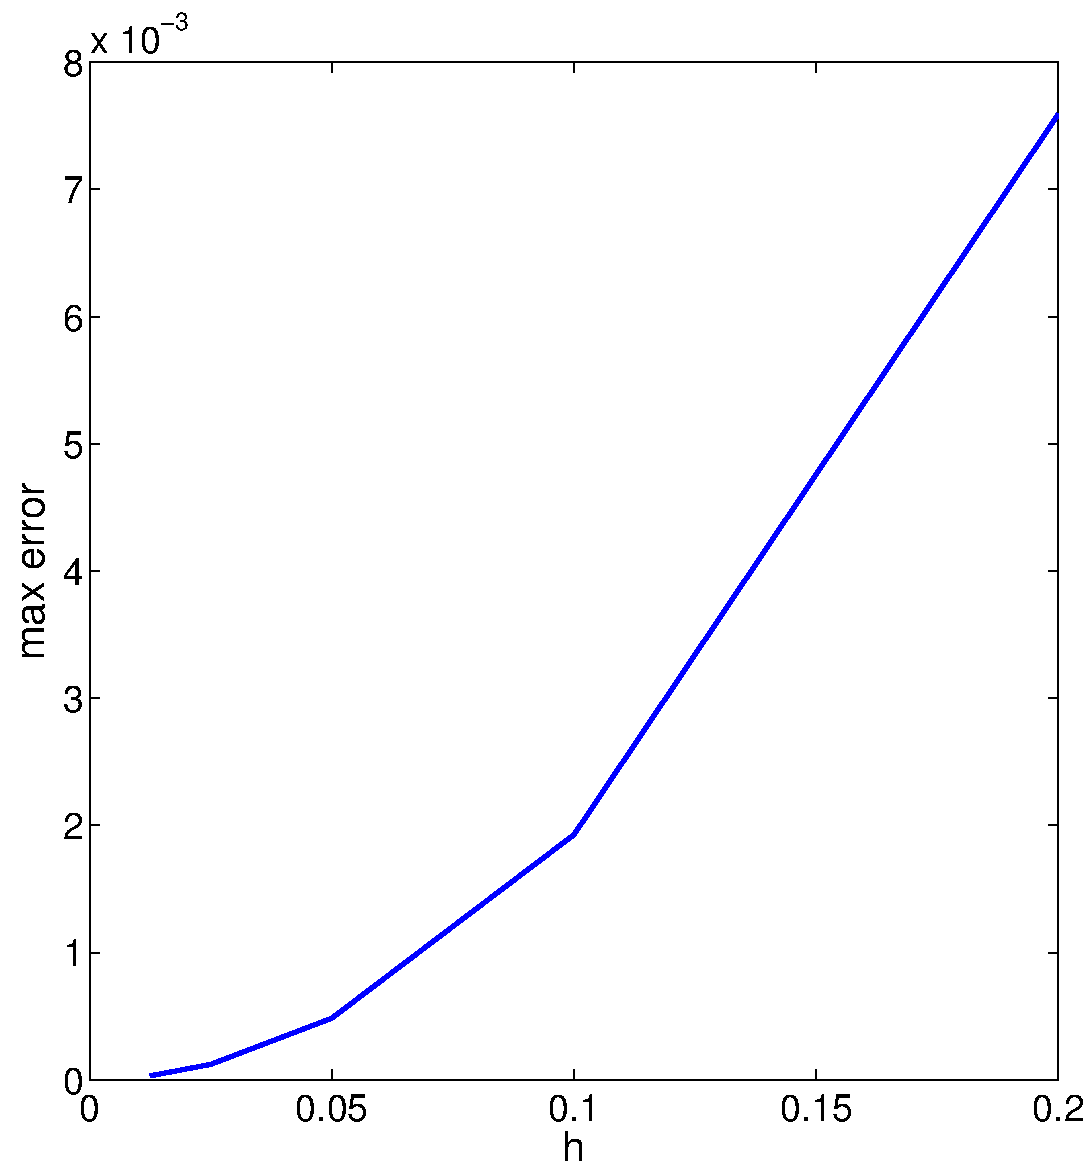
\includegraphics[width=0.5\textwidth]{andy_hw08_prb06_01.pdf}
  \caption{Error in the solution to the BVP with mixed BC at $x = b$, using Method 1 of Sec 8.4, versus $h$.
           We confirm that the method is second order.}
\end{figure}

\begin{figure}[h!]
  \centering
    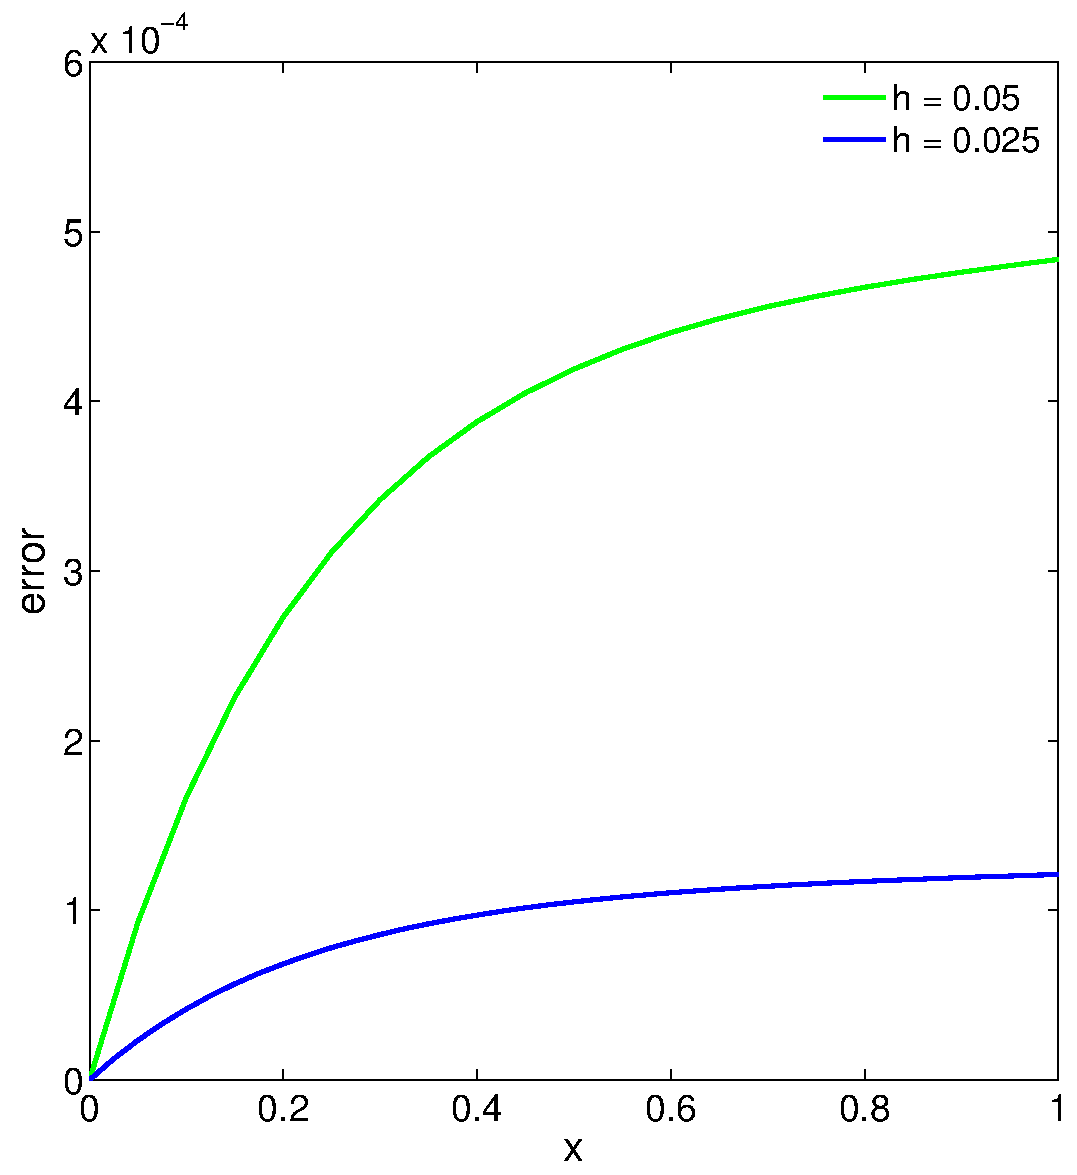
\includegraphics[width=0.5\textwidth]{andy_hw08_prb06_02.pdf}
  \caption{Error in the solution to the BVP with mixed BC at $x = b$, using Method 1 of Sec 8.4, versus $x$ for two values of $h$.}
\end{figure}

\clearpage
\pagebreak
\item Show that if condition (8.42) and the two conditions stated one line below it hold, then the coefficient matrix in Method 2 based on Eq. (8.39) is SDD.

Bonus part: Equations (8.36) and (8.39) each lead to a second-order accurate method.
Therefore, solutions obtained by those methods must differ by $\oh{3}$.
Show {\em analytically} that this is indeed the case.

\bigskip
\textbf{Solution:} Condition (8.42) is that 
\[ A_1 A_2 \leq 0 \]
meaning that they are of opposite parity.
The other conditions ($Q \leq 0, h\mathcal{P} \leq 2$) will also be used.
Consider that the only change in the coefficient matrix from using Method 2, from the form of the original triadiagonal matrix (8.6) is the first row.

To retain SDD of the coefficient matrix, we therefore require that the entry in row 1, column 1 is greater than the entry in row 1, column 2.
Those entries are the coefficients on $Y_{0,1}$, which appear in equation (8.39).
Taking the hint, I begin by multiplying (8.39) by $h/A_2$.
This yeilds:
\[ hY_0 \f{A_1}{A_2} + Y_1 -Y_0 -\f{h^2}{2} R_0 +\f{h}{2} P_0 Y_1 - \f{h}{2} P_0 Y_0+ \f{h^2}{2} Q_0 Y_0 = \f{\alpha h}{A_2} \]
The terms in $Y_0$ and $Y_1$ are thus
\begin{align*} & Y_0: ~~ h\f{A_1}{A_2} - 1 - \f{h}{2} P_0 + \f{h^2}{2} Q_0\\
 & Y_1: ~~ 1+\f{h}{2} P_0 \end{align*}
Now to show that the maginude of the $Y_0$ terms is greater than the magnitude of the $Y_1$ terms, we have (note we drop the inequality since every term is positive by Condition 8.42 and the other conditions)
\begin{align*} \left | h\f{A_1}{A_2} - 1 - \f{h}{2} P_0 + \f{h^2}{2} Q_0 \right | & =\left | \left (1 +\f{h}{2} P_0 \right )- h\f{A_1}{A_2}   - \f{h^2}{2} Q_0 \right |\\
& = \left ( 1+\f{h}{2} P_0\right)   - h\f{A_1}{A_2}- \f{h^2}{2} Q_0\\
& >  1+\f{h}{2} P_0 \\
& = \left | 1+\f{h}{2} P_0 \right |,\end{align*}
which is the magnitude of the coefficient on $Y_1$, as desired.

\clearpage
\pagebreak
\item Solve the BVP stated in Problem 5 of HW 7 using Picard iterations.

\bigskip
\textbf{Solution:} Plot and solution code follow.

The number of iterations does not appear to depend on $h$, nor does the convergence.
For both values of $h$, the shallow solution converges while the deep solution diverges.
The convergence of the shallow solution is achieved in 11 iterations for each $h$.

\lstinputlisting[language=Matlab]{andy_hw08_prb08.m}

\begin{figure}[h!]
  \centering
    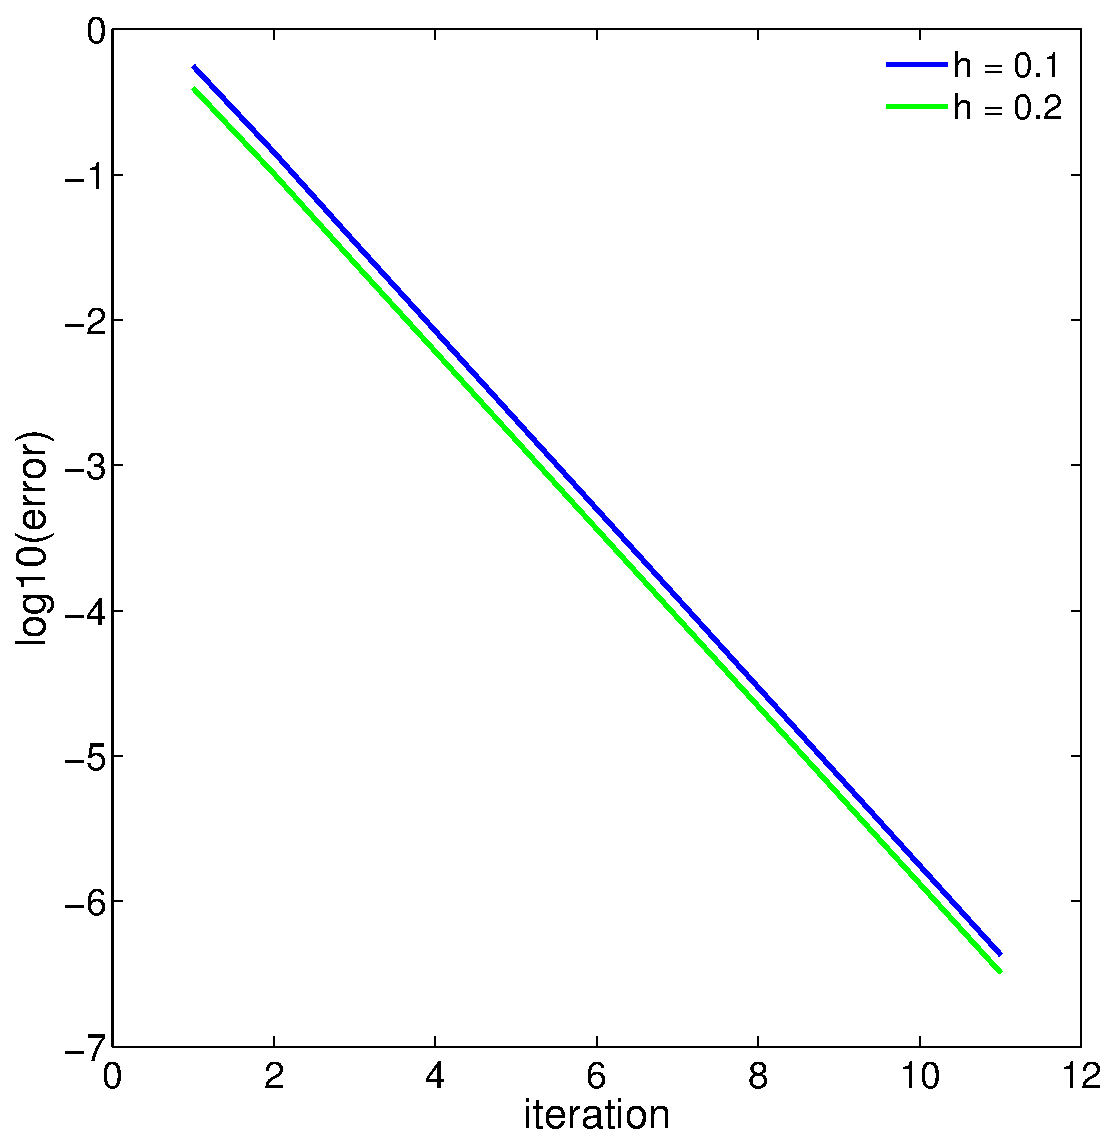
\includegraphics[width=0.45\textwidth]{andy_hw08_prb08_shallowerror.pdf}
  \caption{Logarithm of the error versus iteration number for the Picard iterations, starting close to the shallow solution.
           Since this looks like a straight line, we observe that the Picard method converges linearly.}
\end{figure}

\begin{figure}[h!]
  \centering
    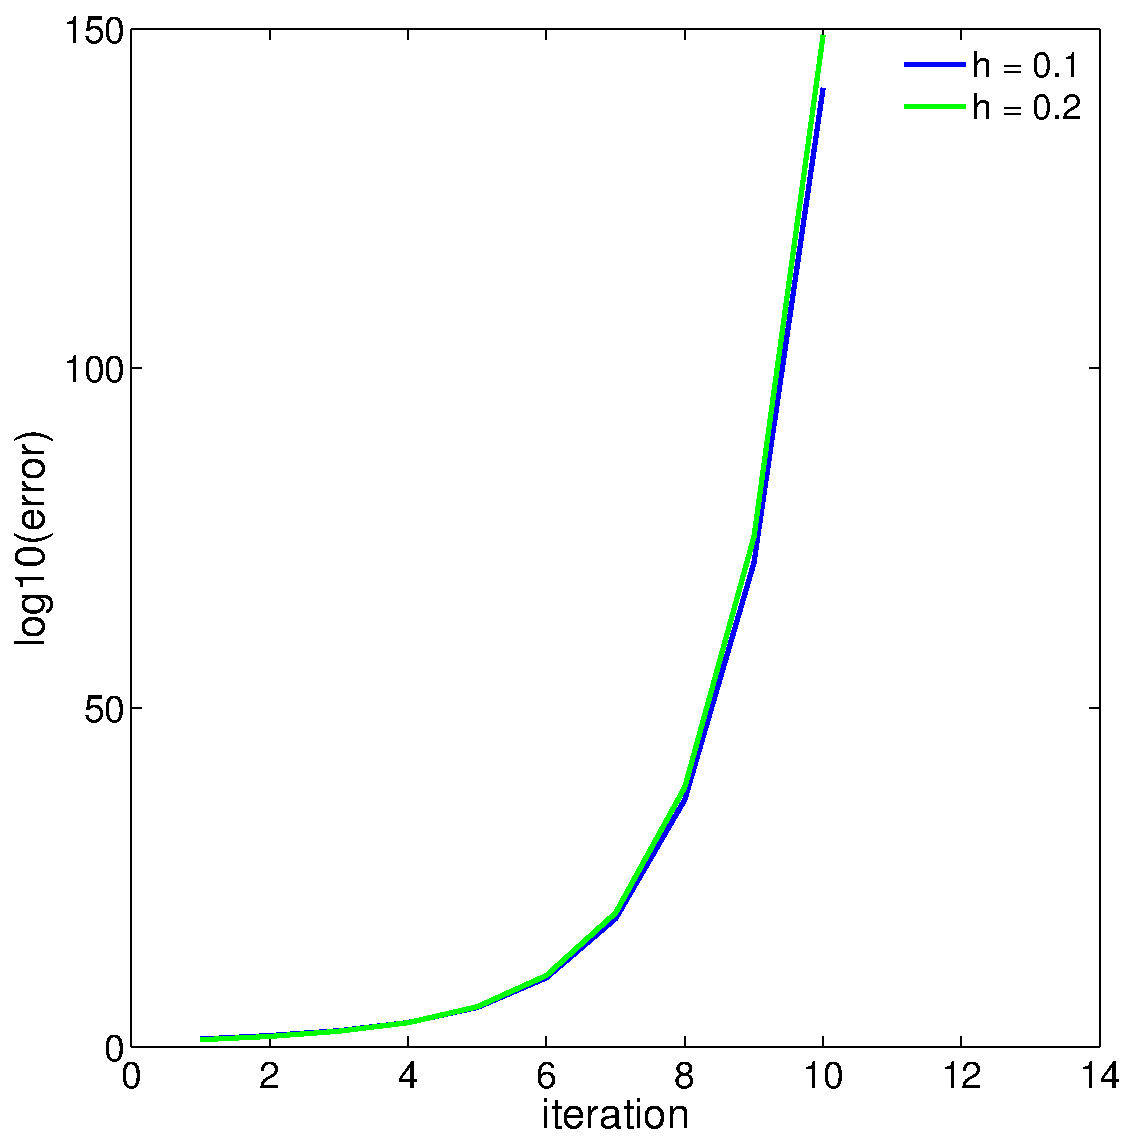
\includegraphics[width=0.45\textwidth]{andy_hw08_prb08_deeperror.pdf}
  \caption{Logarithm of the error versus iteration number for the Picard iterations, starting close to the deep solution.
           The iterations do not converge, and the error runs away.}
\end{figure}

\clearpage
\pagebreak
\item Repeat Problem 8 using the modified Picard's iterations.

\bigskip
\textbf{Solution:} Plot and solution code follow.

I present a summary of the results in a table, where under each value of $h$ I report the number of iterations required.
The ``weird'' behavior manifests as an iteration does not converge to the solution, or go off to infinity, but bounces between two (or more) different $y$.
In the case of simple Picard, the solution bounces between two different $y$, and in modified Picard the behavior is more complicated.
This conclusion was arrived at by plotting $y$ at each iterate, as to see the behavior directly.
In the code, setting ``plot'' to 1 in the Picard function shows these plots (it is suggested to lower the maximum iterate count in this case).

\begin{table}[h]
\begin{center}
\begin{tabular}{cccc}
  \hline
  solution type & $c$ & $h=0.1$ & $h=0.2$ \\
  \hline
  \hline
  shallow & 100 & 314 & 204 \\
          & 20 & 77 & 74 \\
          & 10 & 43 & 42 \\
          & 1.5 & 10 & 10 \\
          & 0.75 & 6 & 6 \\
          & 0 & 11 & 11 \\
          & -0.5 & 25 & 24 \\
          & -0.9 & 327 & 416 \\
          & -1 & --* & --* \\
          & -1.5 & -- & -- \\
  \hline
  deep    & -2.9 & -- & -- \\
          & -4 & 70 & 57 \\
          & -3.9 & 335 & 162 \\
          & -3.75 & --* & --* \\
          & -3.62 & --* & --* \\
          & -3.6 & --* & --* \\
          & -3.55 & --* & --* \\
          & -3.5 & -- & --* \\
          & -5.95 & 22 & 24 \\
          & -6.45 & 42 & 54 \\
          & -6.95 & 933 & 25 \\
          & -7.45 & 13 & 11 \\
  \hline
  deeper  & -4 & -- & -- \\
          & -3.9 & -- & -- \\
          & -5.95 & 24 & 26 \\
          & -6.45 & 46 & 59 \\
          & -6.95 & -- & -- \\
          & -7.45 & -- & -- \\
\end{tabular}
\caption{The iteration count for convergence of Modified Picard to the BVP in Problem 5 of HW7.
         The -- denotes where the solution explodes (runs off the inifinity), and --* where the solution does not converge, but remains bounded.}
\end{center}
\end{table}

\begin{figure}[h!]
  \centering
    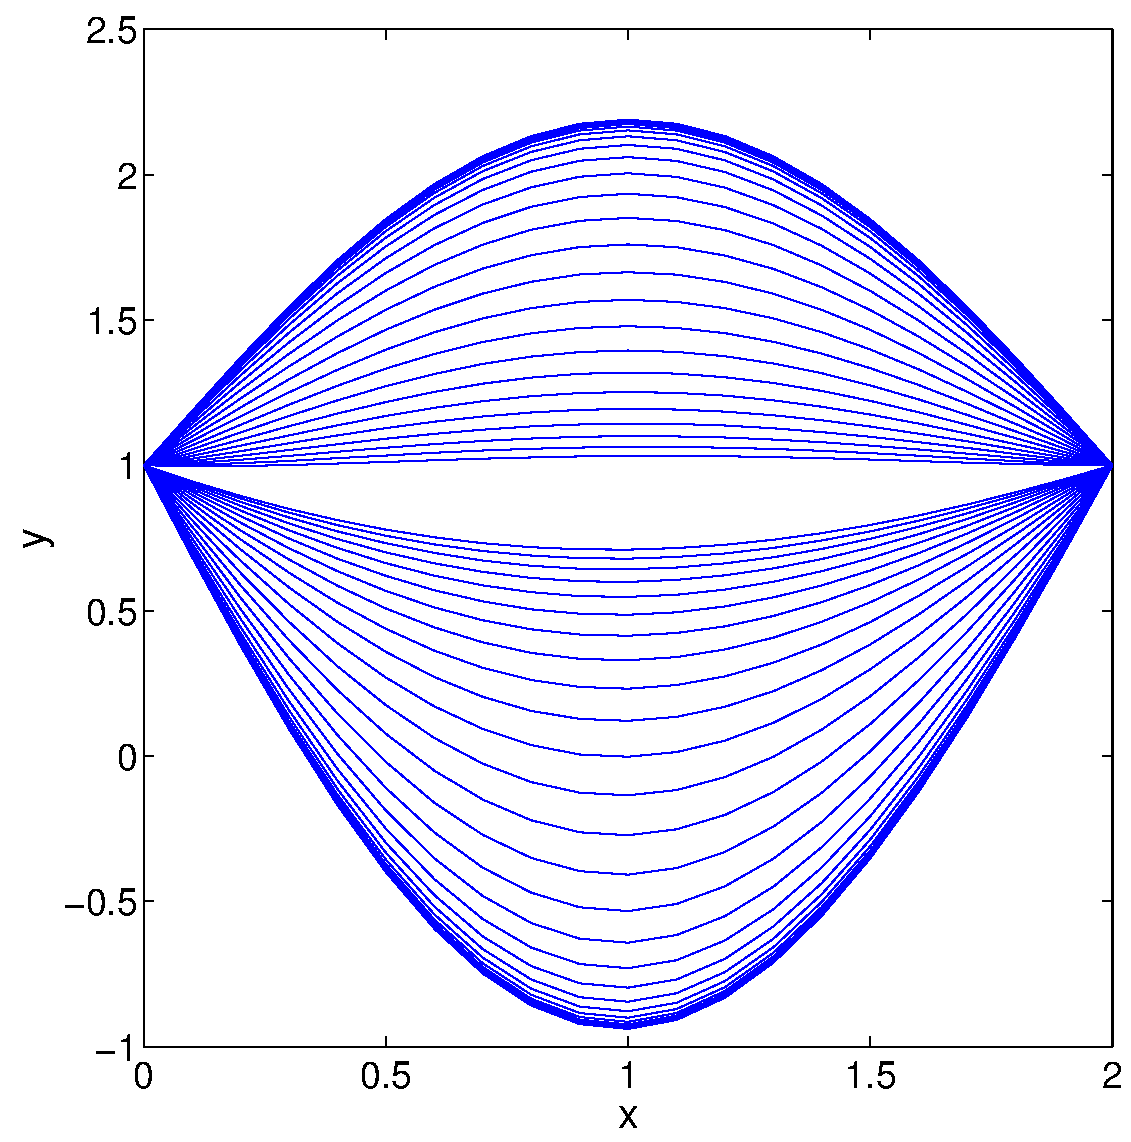
\includegraphics[width=0.45\textwidth]{andy_hw08_prb09_illustrative.pdf}
  \caption{A plot of the iterations in a bounded orbit of length two. The iterations alternate between the top and bottom solutions.}
\end{figure}


%% My code ran, but it only had $c=1$, and found a period two point (but most diverged).
%% Corrected that, and almost everything diverged but for one $h$ and $c = 0.75$ the solution converged to the wrong value, and converged at $c=0$ for both $h$.

%% I would expect convergence at least at $c=0$ since this corresponds to the original Picard's iterations, which converged for both $h$ on the shallow solution.

%% I haven't explored the deep solution considerably, because I wanted to find this ``unexpected'' behavior in the shallow solution, and now I've lost confidence that my code is correct.

\lstinputlisting[language=Matlab]{andy_hw08_prb09.m}

\clearpage
\pagebreak
\item Repeat Problem 8 using the Newton-Raphson method.
Answer all of the questios posed in Problem 8.
As for the logarithm of the error versus the iteration count, you should obtain a parabola facing downward.
Thus, the Newton-Raphson method converges (when it does so) {\em quadratically}.
Is the type of convergence asymptomatically faster or slower than the linear convergence of Picard's methods?

\bigskip
\textbf{Solution:} Plot and solution code follow. I adapt the code from Problem 8, where the only differences are the construction of the matrix $A$ at each iteration, the $r$ vector, and that the result of the matrix solver is the error, which is subtracted for a new solution (it is not the new solution itself).

The number of iterations does not appear to depend on $h$, nor does the convergence.
For both values of $h$, both solutions converge.
The convergence of the shallow solution is achieved in 3 iterations for each $h$, and the deep solution in 5 iterations.

\lstinputlisting[language=Matlab]{andy_hw08_prb10.m}

\begin{figure}[h!]
  \centering
    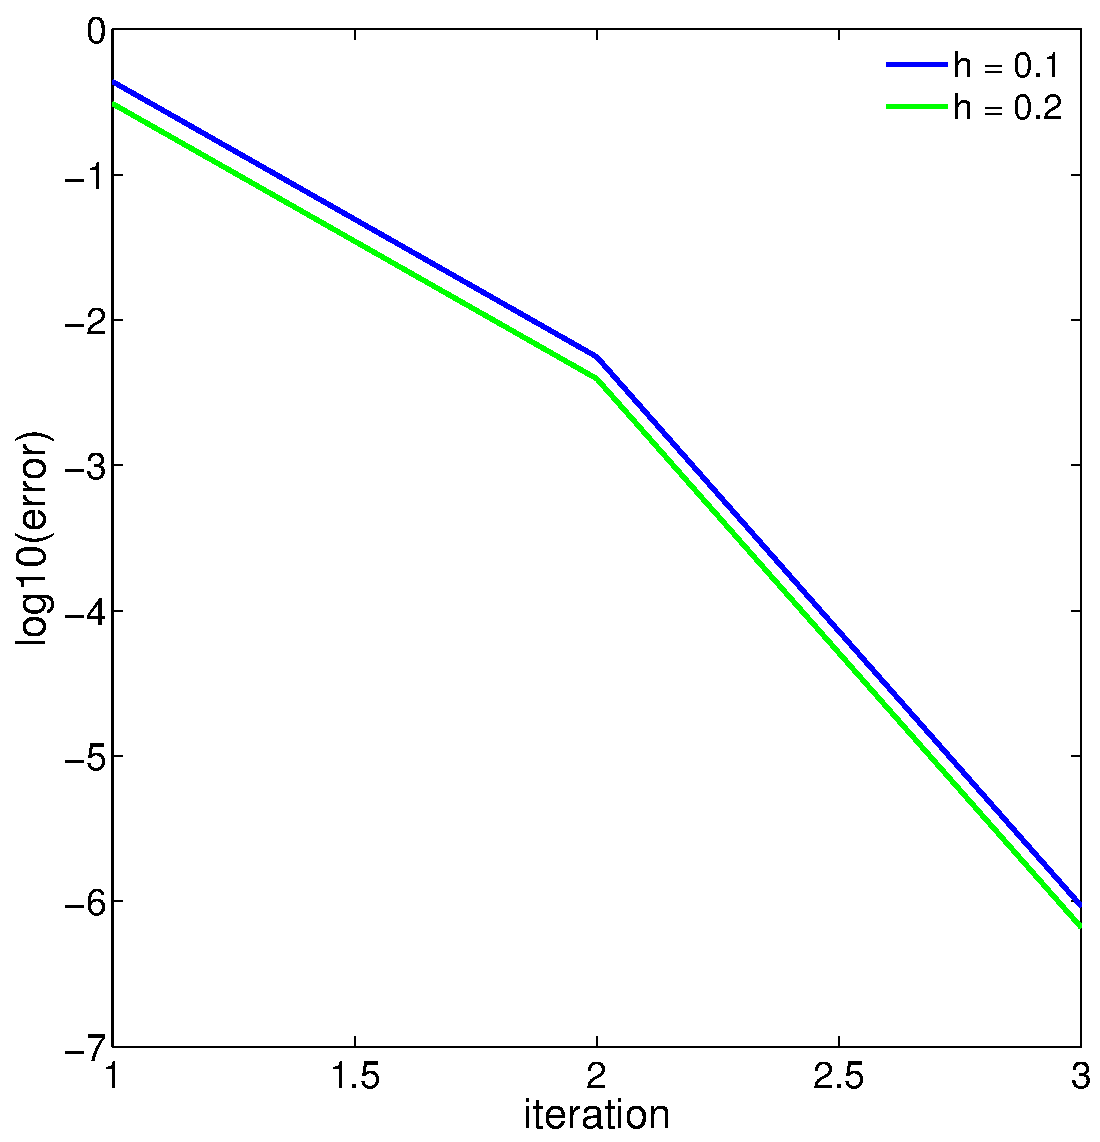
\includegraphics[width=0.45\textwidth]{andy_hw08_prb10_shallowerror.pdf}
  \caption{Logarithm of the error versus iteration number for the Picard iterations, starting close to the shallow solution.
           Since this looks like a straight line, we observe that the Picard method converges linearly.}
\end{figure}

\begin{figure}[h!]
  \centering
    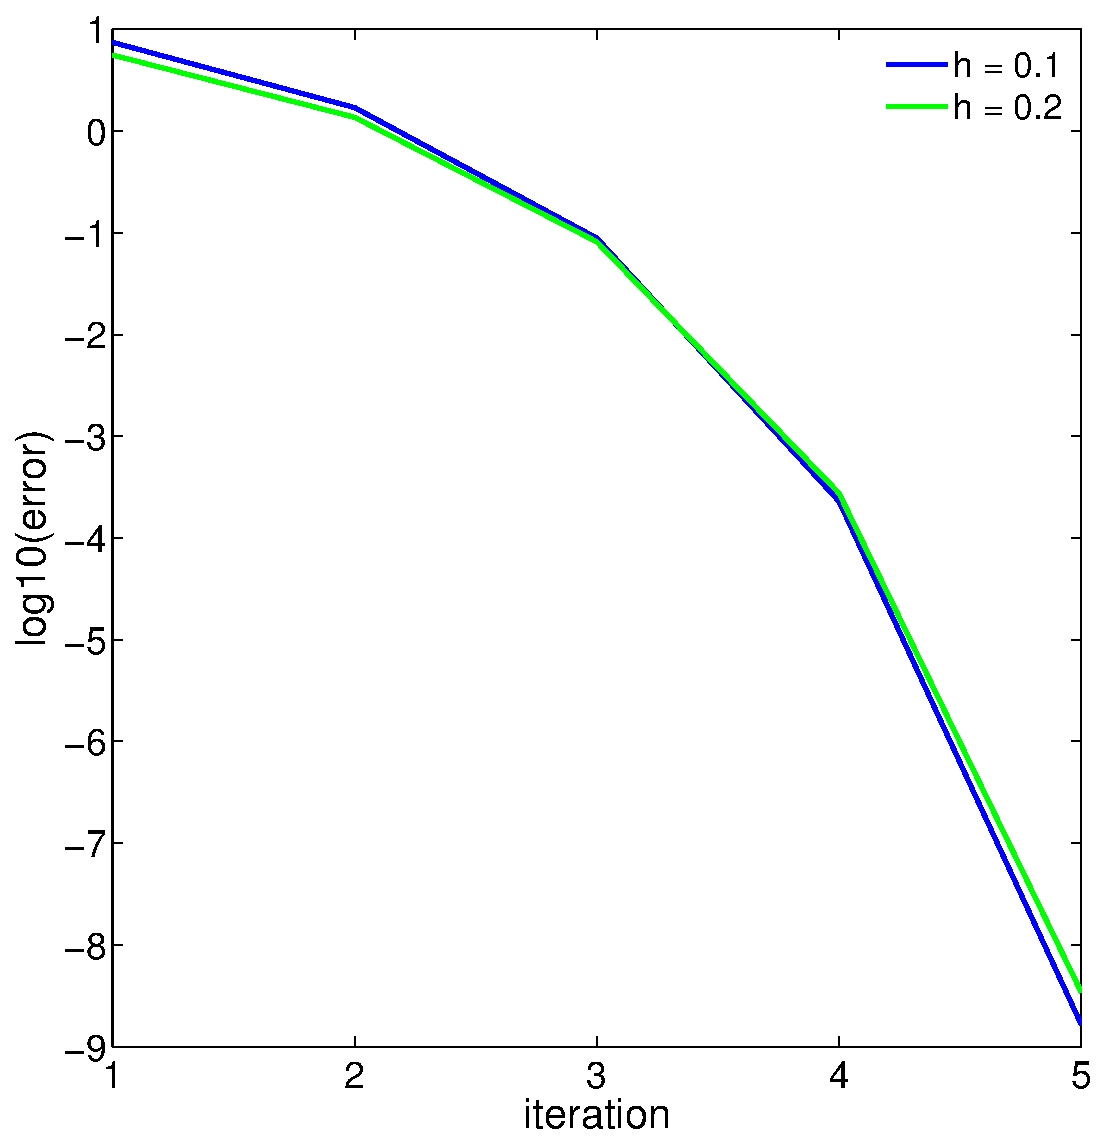
\includegraphics[width=0.45\textwidth]{andy_hw08_prb10_deeperror.pdf}
  \caption{Logarithm of the error versus iteration number for the Picard iterations, starting close to the deep solution.
           The iterations do not converge, and the error runs away.}
\end{figure}

\clearpage
\pagebreak
\item Compare  your results in Problems 8-10 and draw conclusions.
Namely, based on your experience with the previous three problems, list strengths and weaknesses for each of the three methods.
Then explain under which circumstances you would and would not use, each of these methods.

\bigskip
\textbf{Solution:} 
\begin{table}[h]
\begin{center}
\begin{tabular}{lll}
  \hline
  method & strengths & weaknesses \\
  \hline
  \hline
  Picard & easy to code & cannot obtain deep solution\\
         & & linear convergence\\
  \hline
  modifid Picard & can obtain both solutions & linear convergence\\
            & not too hard to code & very sensitive to $c$\\
  \hline
  Newton-Raphson & very fast (quad. conv.) & \\
            & not too hard to code & \\
            & obtains both solutions & \\
  \hline
\end{tabular}
\caption{The strengths and weaknesses of the BVP iteration schemes tested.}
\end{center}
\end{table}
\end{enumerate}

\clearpage
\pagebreak
{\huge Appendix 1: ODE Functions}
\lstinputlisting[language=Matlab]{andy_hw07_prb05_ODE.m}
%% \lstinputlisting[language=Matlab]{andy_hw08_prb01_ODEh.m}

\clearpage
\pagebreak
{\huge Appendix 2: Numerical Methods}

\lstinputlisting[language=Matlab]{andy_hw08_prb08_r.m}
\lstinputlisting[language=Matlab]{andy_hw08_prb09_picard.m}
\lstinputlisting[language=Matlab]{andy_hw08_prb10_r.m}
%% \lstinputlisting[language=Matlab]{andy_MEr.m}

\end{document}



